\documentclass[UTF8,a4paper,12pt]{ctexart}

\usepackage{amsmath,amssymb}
\usepackage{booktabs}
\usepackage{caption}
\usepackage{float}
\usepackage{geometry}
\usepackage{graphicx}
\usepackage{hyperref}
\usepackage{longtable}
\usepackage{xcolor}
\usepackage{enumitem}
\usepackage{fvextra}

\geometry{left=2.6cm,right=2.6cm,top=2.6cm,bottom=2.6cm}
\hypersetup{colorlinks=true,linkcolor=black,urlcolor=blue}
\setlength{\parindent}{2em}
\setlength{\parskip}{0.25em}
\setlength{\emergencystretch}{3em}
\sloppy
\linespread{1.25}
\setlist[itemize]{leftmargin=2.5em,itemsep=0.15em}
\DefineVerbatimEnvironment{CodeBlock}{Verbatim}{breaklines,breakanywhere,fontsize=\small,frame=single,rulecolor=\color{gray!45}}

\title{\heiti 机器学习与Python实践\\[0.8em]\Large 第3次作业\\[1.6em]\Huge 基于汽油类型的汽车油耗预测模型}
\author{}
\date{}

\begin{document}

\begin{titlepage}
    \centering
    \vspace*{1.2cm}
    
\includegraphics[width=0.78\linewidth]{figures/cover_logo.png}\par
    \vspace{1.0cm}
    {\zihao{2}\heiti 机器学习与Python实践\par}
    \vspace{0.8cm}
    {\zihao{3}\heiti 第3次作业\par}
    \vspace{1.2cm}
    {\zihao{1}\heiti 基于汽油类型的汽车油耗预测模型\par}
    \vfill
    \begin{tabular}{rl}
        姓名：& 匿名\\[0.45em]
        专业：& 强基班\\[0.45em]
        学号：& \\[0.45em]
        教师：& 匿名\\[0.45em]
        学院：& 信息科学与工程学院\\[0.45em]
    \end{tabular}
    \vfill
    {\zihao{4}2026年5月25日\par}
\end{titlepage}

\tableofcontents
\newpage

\section{前言及问题概述}

汽车油耗是车辆使用成本和能源效率的重要指标。对于同一辆车，如果行驶路线、驾驶习惯和天气条件较为接近，那么汽油类型、平均速度、行驶距离、车内外温度、是否开空调以及是否下雨等因素都可能影响单位百公里油耗。题目给出的案例中，James 长期驾驶同一辆车，并在加油站交替使用 E10 和 SP98 两类汽油，其中 E10 单价较低，但经验上使用 E10 时车辆耗油量更高。因此，本次实验的核心任务是根据给定行驶记录，建立模型预测汽车油耗 \texttt{consume}，并分析汽油类型在预测中的作用。

本实验使用 \texttt{measurements.xlsx} 数据集，共 388 条样本，包含 11 个输入特征和 1 个目标特征。目标变量为 \texttt{consume}，表示每百公里消耗燃油升数，单位为 L/100km。输入特征包括行驶距离、平均速度、车内温度、车外温度、特殊事件、汽油类型、空调、雨天、晴天、补充汽油升数和补充汽油类型。实验先进行数据预览、缺失值分析和探索性可视化，再构造若干补充特征，最后比较仅使用汽油类型的基线模型、线性回归、岭回归、随机森林回归和梯度提升回归的预测效果。

需要特别说明的是，本题虽然强调“根据汽油类型预测消耗量”，但真实油耗并不只由汽油类型决定。仅使用 \texttt{gas\_type} 建模能够检验汽油类型自身的解释能力，而使用全部行驶和环境特征建模则更接近实际预测场景。两类结果结合起来，可以更清楚地说明汽油类型与油耗之间的关系。

\section{相关基础知识及方法}

\subsection{相关原理}

本任务属于监督学习中的回归问题。设第 $i$ 条行驶记录的输入特征为 $x^{(i)}$，目标油耗为 $y^{(i)}$，回归模型的目标是学习函数 $f(x)$，使预测值
\begin{equation}
    \hat{y}^{(i)}=f(x^{(i)})
\end{equation}
尽可能接近真实油耗。模型效果通过测试集上的误差指标评价。

线性回归假设目标变量与特征之间近似满足线性关系：
\begin{equation}
    \hat{y}=w_0+w_1x_1+\cdots+w_dx_d .
\end{equation}
该模型结构清晰、可解释性强，但对非线性关系和特征交互的表达能力有限。岭回归在线性回归基础上加入 $L_2$ 正则化项，目标函数为
\begin{equation}
    J(\mathbf{w})=\frac{1}{n}\sum_{i=1}^{n}(\hat{y}^{(i)}-y^{(i)})^2+\lambda\|\mathbf{w}\|_2^2 ,
\end{equation}
能够在一定程度上缓解多重共线性和过拟合。

随机森林回归属于集成学习方法。它通过多个决策树在不同样本和特征子集上学习规律，并取多棵树预测结果的平均值：
\begin{equation}
    \hat{y}=\frac{1}{T}\sum_{t=1}^{T}f_t(x).
\end{equation}
与线性模型相比，随机森林能够自动捕捉非线性关系和变量交互，因此适合处理行驶距离、速度、天气和空调等因素共同影响油耗的表格型数据。梯度提升回归同样基于决策树，但采用逐步拟合残差的方式不断提升模型表现。

本实验使用 RMSE、MAE、$R^2$ 和 NRMSE 四个指标评价模型。RMSE 定义为
\begin{equation}
    RMSE=\sqrt{\frac{1}{n}\sum_{i=1}^{n}(\hat{y}^{(i)}-y^{(i)})^2},
\end{equation}
MAE 定义为
\begin{equation}
    MAE=\frac{1}{n}\sum_{i=1}^{n}\left|\hat{y}^{(i)}-y^{(i)}\right|,
\end{equation}
$R^2$ 定义为
\begin{equation}
    R^2=1-\frac{\sum_{i=1}^{n}(y^{(i)}-\hat{y}^{(i)})^2}{\sum_{i=1}^{n}(y^{(i)}-\bar{y})^2}.
\end{equation}
其中 RMSE、MAE 和 NRMSE 越小越好，$R^2$ 越接近 1 表示模型解释能力越强。

\subsection{数据描述}

数据集文件为 \texttt{measurements.xlsx}，读取后共 388 行、12 列，其中 \texttt{consume} 为目标变量，其余 11 列作为候选输入特征。主要字段说明见表 \ref{tab:features}。

\begin{longtable}{lll}
\caption{汽车油耗数据集字段说明}\label{tab:features}\\
\toprule
字段 & 类型 & 含义\\
\midrule
\endfirsthead
\toprule
字段 & 类型 & 含义\\
\midrule
\endhead
\texttt{distance} & 连续特征 & 行车距离，单位 km\\
\texttt{consume} & 目标变量 & 消耗量，单位 L/100km\\
\texttt{speed} & 连续特征 & 平均速度，单位 km/h\\
\texttt{temp\_inside} & 连续特征 & 车内温度，单位 $^\circ$C\\
\texttt{temp\_outside} & 连续特征 & 车外温度，单位 $^\circ$C\\
\texttt{specials} & 类别特征 & 是否发生特殊事件，如雨、阳光、空调等\\
\texttt{gas\_type} & 类别特征 & 使用汽油类型，E10 或 SP98\\
\texttt{AC} & 二值特征 & 是否开启空调\\
\texttt{rain} & 二值特征 & 是否下雨\\
\texttt{sun} & 二值特征 & 是否阳光明媚\\
\texttt{refill\_liters} & 连续特征 & 补充汽油升数\\
\texttt{refill\_gas} & 类别特征 & 补充汽油类型\\
\bottomrule
\end{longtable}

数据中 \texttt{distance}、\texttt{consume}、\texttt{speed}、\texttt{temp\_outside}、\texttt{gas\_type}、\texttt{AC}、\texttt{rain} 和 \texttt{sun} 均无缺失值。\texttt{temp\_inside} 有 12 个缺失值，\texttt{specials} 有 295 个缺失值，\texttt{refill\_liters} 和 \texttt{refill\_gas} 各有 375 个缺失值。由于补油字段缺失数量很高，缺失本身也包含“本次记录没有补油信息”的含义，因此实验没有直接删除这些样本，而是将类别缺失填充为 \texttt{none}，数值缺失使用中位数填充，并额外构造 \texttt{has\_refill} 和 \texttt{has\_special} 两个二值特征。

目标变量 \texttt{consume} 的均值为 4.9124，标准差为 1.0332，最小值为 3.3，最大值为 12.2。不同汽油类型下的油耗统计见表 \ref{tab:gasstat}。

\begin{table}[H]
\centering
\caption{不同汽油类型下的油耗统计}
\label{tab:gasstat}
\begin{tabular}{lrrrrrr}
\toprule
汽油类型 & 样本数 & 均值 & 中位数 & 标准差 & 最小值 & 最大值\\
\midrule
E10 & 160 & 4.9313 & 4.8000 & 0.9010 & 3.7 & 10.8\\
SP98 & 228 & 4.8991 & 4.7000 & 1.1184 & 3.3 & 12.2\\
\bottomrule
\end{tabular}
\end{table}

从表中可以看到，E10 的平均油耗略高于 SP98，但差异仅约 0.032 L/100km，远小于样本自身波动。因此，汽油类型可能提供一定信息，但很难单独解释油耗变化。

\begin{figure}[H]
    \centering
    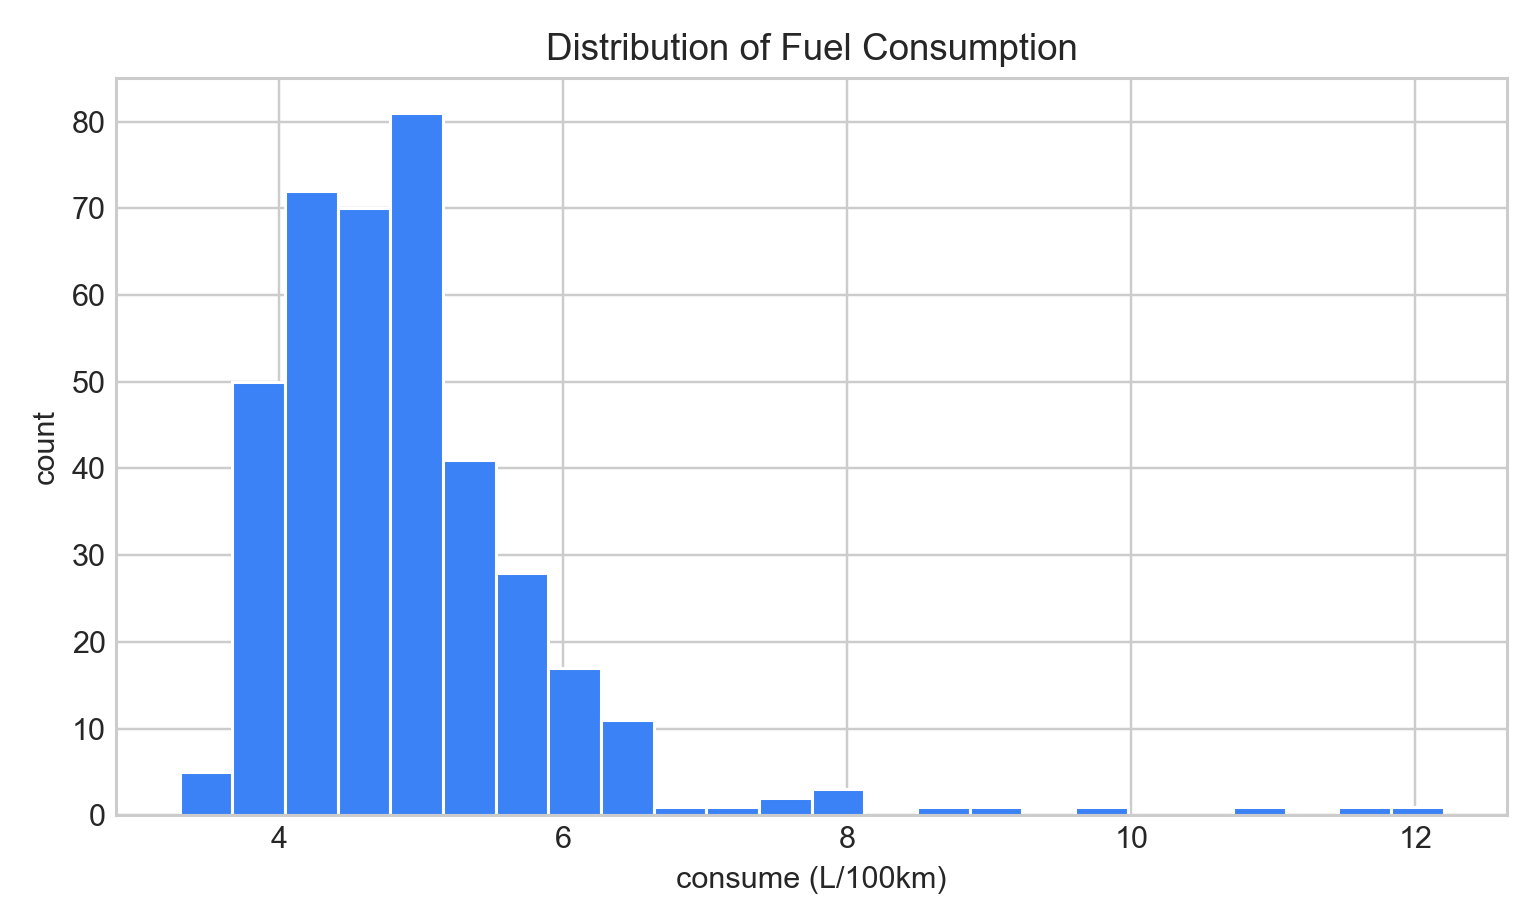
\includegraphics[width=0.78\linewidth]{figures/target_consume_distribution.png}
    \caption{目标变量 \texttt{consume} 分布}
    \label{fig:targetdist}
\end{figure}

\begin{figure}[H]
    \centering
    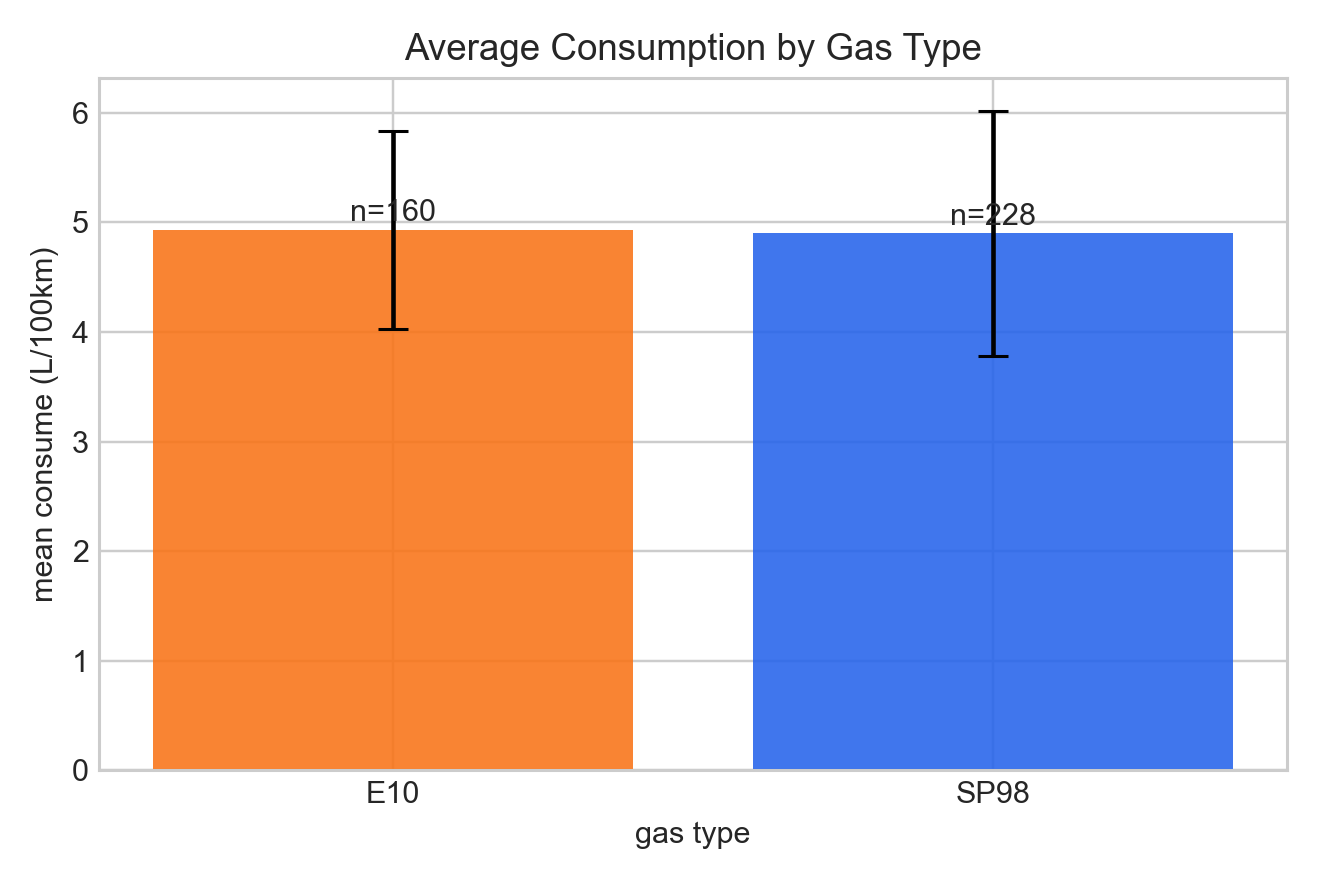
\includegraphics[width=0.72\linewidth]{figures/consume_by_gas_type.png}
    \caption{不同汽油类型的平均油耗}
    \label{fig:gasbar}
\end{figure}

\subsection{算法实现}

实验程序使用 \texttt{pandas} 读取 Excel 数据，使用 \texttt{scikit-learn} 完成预处理、模型训练和模型评价。主要流程如下：

\begin{enumerate}
    \item 读取 \texttt{measurements.xlsx}，确认数据规模、字段类型、缺失值和描述性统计。
    \item 对 \texttt{gas\_type} 分组统计平均油耗，并绘制目标变量分布、汽油类型油耗柱状图、速度与油耗散点图和相关性热力图。
    \item 构造 \texttt{has\_special}、\texttt{has\_refill}、\texttt{temp\_diff\_inside\_outside}、\texttt{distance\_per\_speed}、\texttt{speed\_temp\_interaction} 等补充特征。
    \item 将数据按 80\%/20\% 随机划分为训练集和测试集，其中训练集 310 条，测试集 78 条。
    \item 对数值特征使用中位数填充并进行标准化，对类别特征使用常量 \texttt{none} 填充后进行 One-Hot 编码。
    \item 分别训练 \texttt{GasType\_LinearRegression}、\texttt{Full\_LinearRegression}、\texttt{Full\_Ridge}、\texttt{Full\_RandomForest} 和 \texttt{Full\_GradientBoosting} 五个模型。
    \item 在测试集上计算 RMSE、MAE、$R^2$ 和 NRMSE，同时使用 5 折交叉验证估计模型稳定性。
    \item 保存最佳模型的真实值与预测值散点图、预测曲线以及随机森林特征重要性图。
\end{enumerate}

完整 Python 程序见附录。

\section{实验结果与可扩展内容}

\subsection{实验结果}

图 \ref{fig:speedscatter} 展示了平均速度和油耗之间的关系。总体上，速度较低时油耗更容易偏高，这符合车辆低速行驶、频繁启停时燃油效率较低的经验。两类汽油样本在散点图中存在较多重叠，也说明汽油类型并不是唯一主导因素。

\begin{figure}[H]
    \centering
    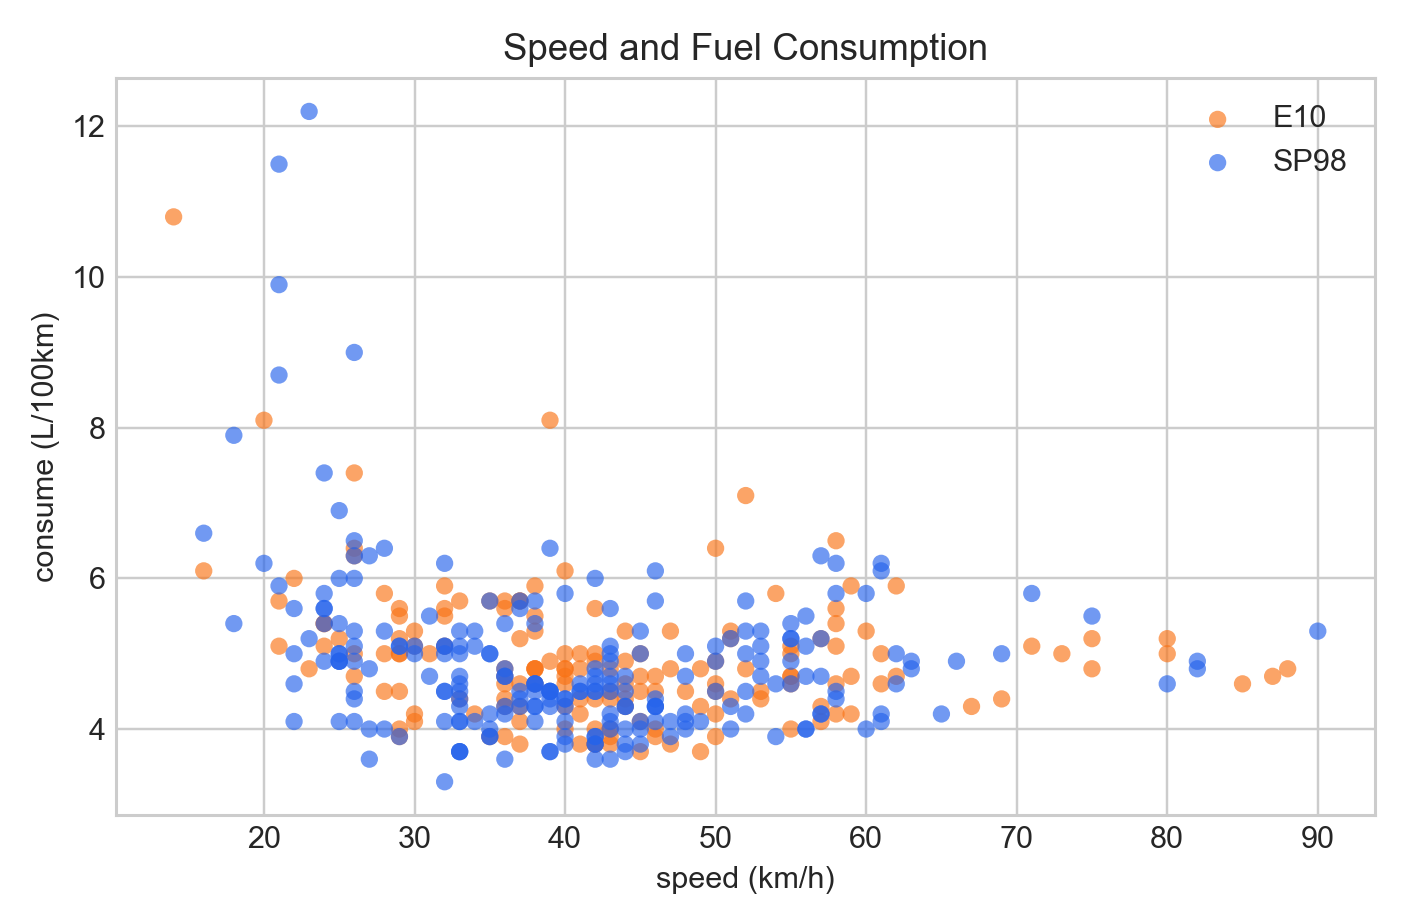
\includegraphics[width=0.82\linewidth]{figures/speed_vs_consume.png}
    \caption{平均速度与油耗的关系}
    \label{fig:speedscatter}
\end{figure}

数值特征相关性热力图见图 \ref{fig:corr}。与目标变量 \texttt{consume} 关系较明显的是 \texttt{distance}、\texttt{speed}、\texttt{rain} 和 \texttt{AC} 等字段。其中行驶距离与油耗呈负相关，说明短距离行驶更容易出现较高单位油耗；平均速度与油耗也呈负相关，反映出低速或拥堵环境下油耗更高。

\begin{figure}[H]
    \centering
    
\includegraphics[width=0.9\linewidth]{figures/correlation_heatmap.png}
    \caption{数值特征相关性热力图}
    \label{fig:corr}
\end{figure}

不同模型在测试集上的结果见表 \ref{tab:modelresult}。仅使用汽油类型的线性回归模型 \texttt{GasType\_LinearRegression} 测试集 $R^2$ 仅为 0.0023，几乎不能解释油耗波动。这与前文分组统计一致，说明 E10 与 SP98 的平均油耗差异较小，单独使用汽油类型预测不足以得到可靠模型。

\begin{table}[H]
\centering
\caption{模型测试集评价结果}
\label{tab:modelresult}
\begin{tabular}{lrrrr}
\toprule
模型 & RMSE & MAE & $R^2$ & NRMSE\\
\midrule
\texttt{Full\_RandomForest} & 0.6567 & 0.4285 & 0.5247 & 0.1042\\
\texttt{Full\_GradientBoosting} & 0.8041 & 0.4770 & 0.2874 & 0.1276\\
\texttt{Full\_LinearRegression} & 0.8513 & 0.6271 & 0.2012 & 0.1351\\
\texttt{Full\_Ridge} & 0.8558 & 0.6302 & 0.1928 & 0.1358\\
\texttt{GasType\_LinearRegression} & 0.9514 & 0.6396 & 0.0023 & 0.1510\\
\bottomrule
\end{tabular}
\end{table}

加入全部行驶和环境特征后，模型效果明显提升。其中随机森林表现最好，测试集 RMSE 为 0.6567，MAE 为 0.4285，$R^2$ 为 0.5247，说明模型能够解释约 52.47\% 的测试集油耗波动。梯度提升模型次之，线性回归和岭回归低于树模型，说明本数据中存在一定非线性关系和特征交互。

表 \ref{tab:cvresult} 给出了 5 折交叉验证平均结果。随机森林的交叉验证 RMSE 为 0.6836，平均 $R^2$ 为 0.4964，与测试集结果较接近，说明模型表现具有一定稳定性。

\begin{table}[H]
\centering
\caption{模型 5 折交叉验证结果}
\label{tab:cvresult}
\begin{tabular}{lrrr}
\toprule
模型 & CV RMSE均值 & CV MAE均值 & CV $R^2$均值\\
\midrule
\texttt{Full\_RandomForest} & 0.6836 & 0.4525 & 0.4964\\
\texttt{Full\_GradientBoosting} & 0.7244 & 0.4898 & 0.4308\\
\texttt{Full\_LinearRegression} & 0.9942 & 0.6494 & -0.0384\\
\texttt{Full\_Ridge} & 0.9681 & 0.6473 & 0.0087\\
\texttt{GasType\_LinearRegression} & 1.0153 & 0.6756 & -0.0485\\
\bottomrule
\end{tabular}
\end{table}

最佳模型的预测效果见图 \ref{fig:predscatter} 和图 \ref{fig:predcurve}。从散点图看，随机森林的多数预测点靠近理想预测直线，但对于个别高油耗样本仍存在低估现象。这与数据集中高油耗样本数量较少有关，模型更容易学习到常见油耗范围内的规律。

\begin{figure}[H]
    \centering
    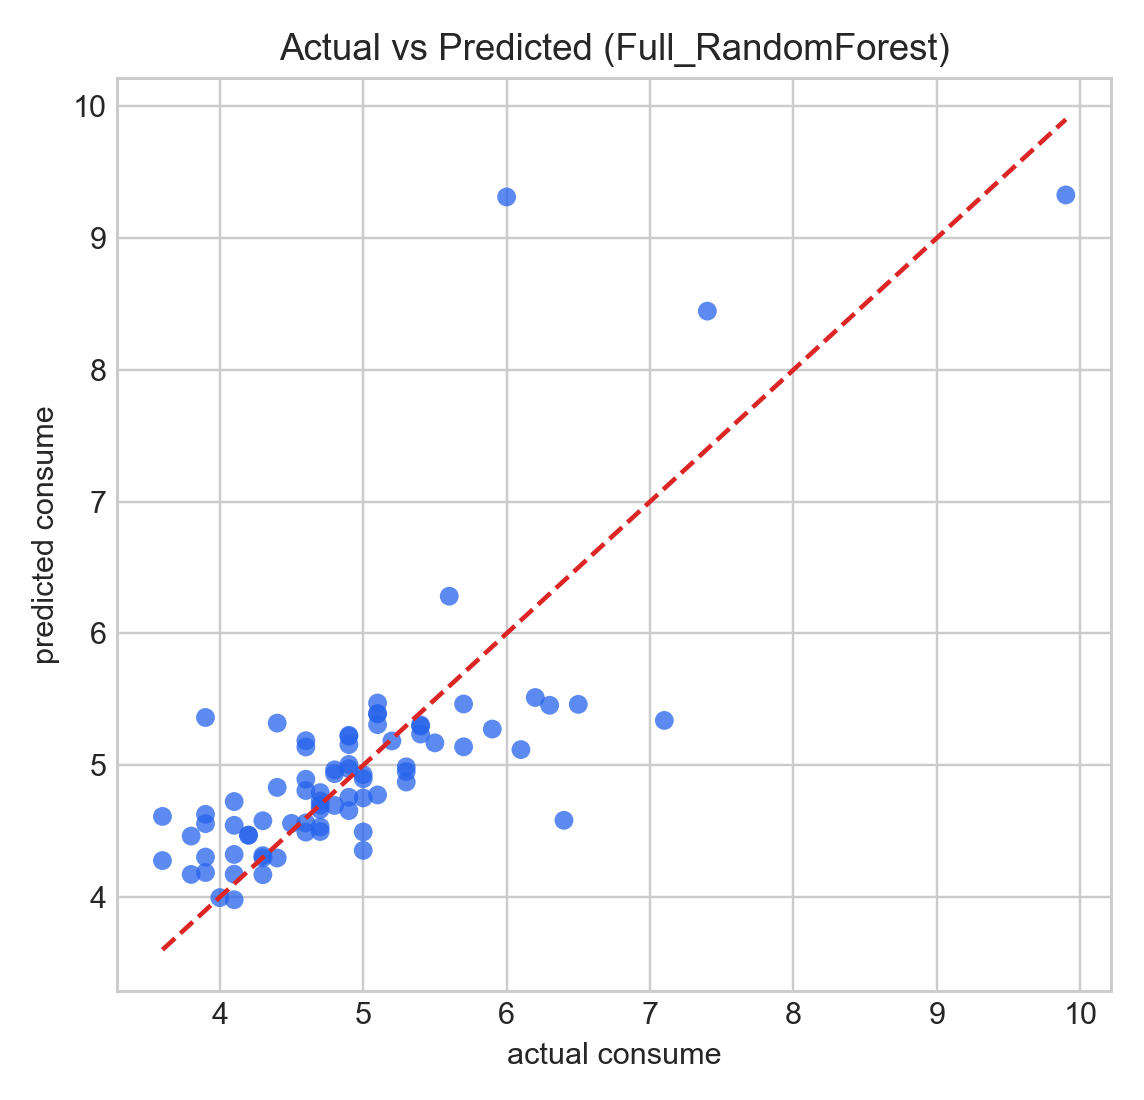
\includegraphics[width=0.68\linewidth]{figures/best_prediction_scatter.png}
    \caption{最佳模型真实值与预测值散点图}
    \label{fig:predscatter}
\end{figure}

\begin{figure}[H]
    \centering
    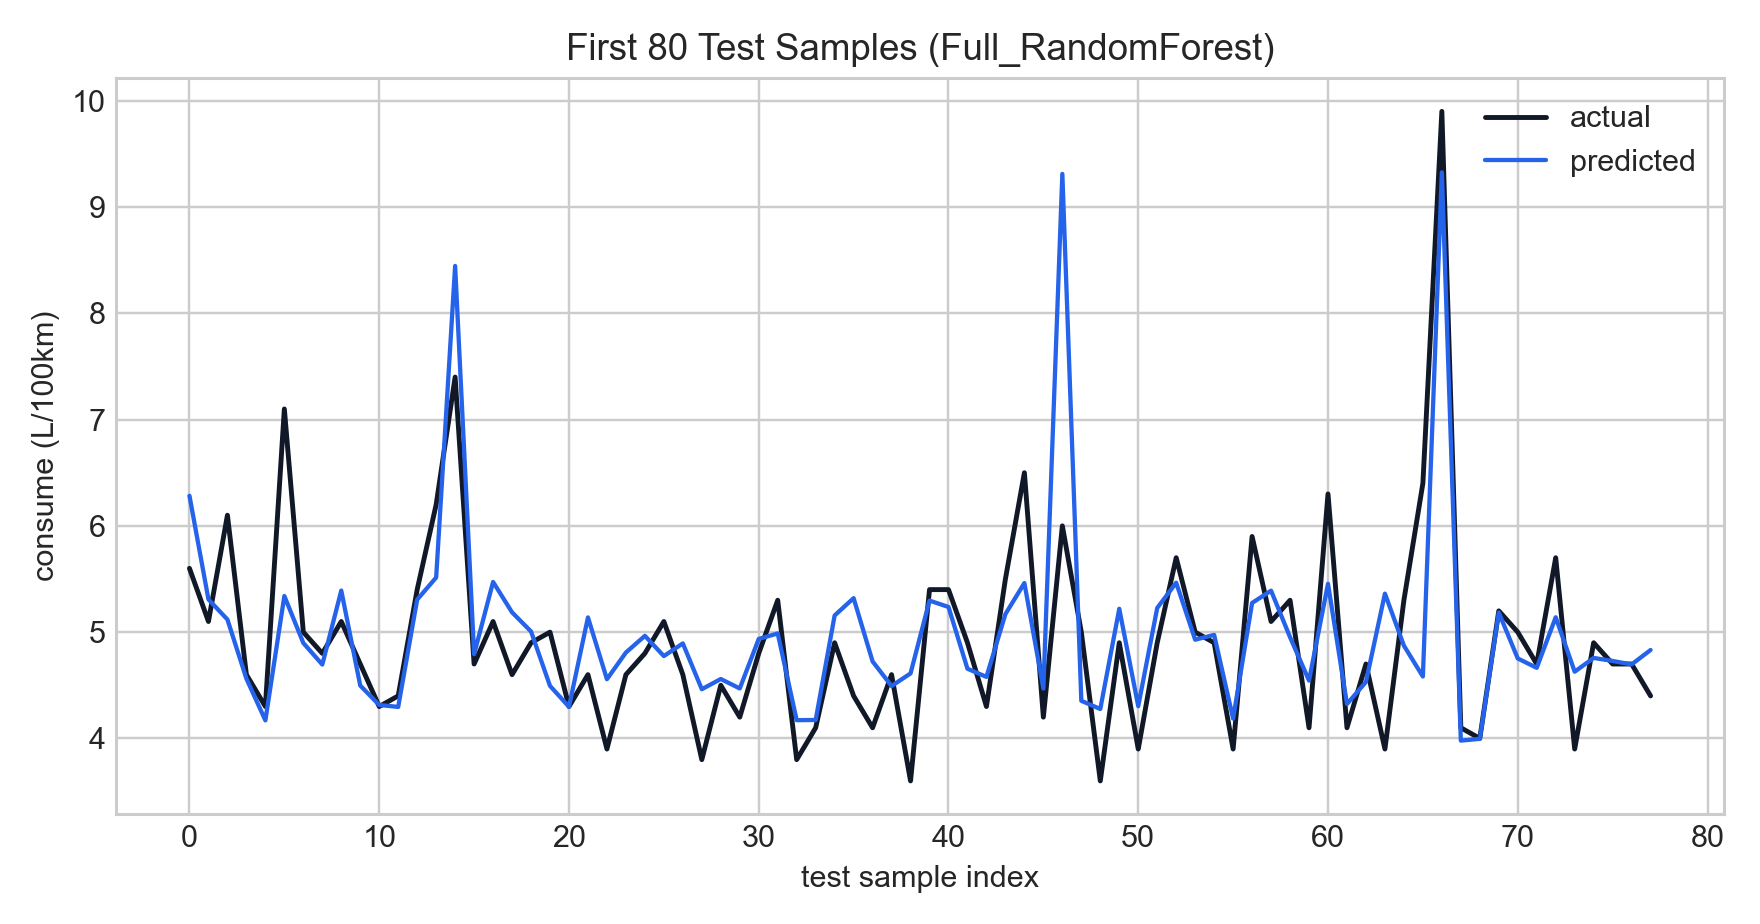
\includegraphics[width=0.9\linewidth]{figures/best_prediction_curve.png}
    \caption{最佳模型测试集前 80 个样本预测曲线}
    \label{fig:predcurve}
\end{figure}

随机森林特征重要性见图 \ref{fig:importance}。结果显示，\texttt{distance} 的重要性最高，为 0.5014；其次是 \texttt{distance\_per\_speed}、\texttt{speed\_temp\_interaction}、\texttt{speed} 和 \texttt{temp\_outside}。与之相比，\texttt{gas\_type\_SP98} 和 \texttt{gas\_type\_E10} 的重要性分别约为 0.0021 和 0.0020，说明在当前数据和模型中，汽油类型对油耗预测的贡献较小，行驶状态和环境因素更关键。

\begin{figure}[H]
    \centering
    
\includegraphics[width=0.9\linewidth]{figures/feature_importance_top20.png}
    \caption{随机森林前 20 个重要特征}
    \label{fig:importance}
\end{figure}

\subsection{参数调优及可扩展内容}

本次实验使用固定参数完成模型比较。随机森林设置为 500 棵树，最小叶节点样本数为 3，以降低小样本数据上的过拟合风险。梯度提升模型设置 180 棵树、学习率为 0.04、树深为 3。后续若继续优化，可以从以下方向扩展：

\begin{itemize}
    \item 使用网格搜索或随机搜索调节随机森林的 \texttt{max\_depth}、\texttt{min\_samples\_leaf} 和 \texttt{max\_features}。
    \item 对梯度提升模型进一步搜索 \texttt{n\_estimators}、\texttt{learning\_rate} 和 \texttt{subsample}，在偏差和方差之间取得更好平衡。
    \item 加入更贴近驾驶场景的特征，例如短距离行驶标记、低速行驶标记、雨天且开空调交互、温差分箱等。
    \item 若后续有时间顺序或路线信息，可以构造滚动平均油耗、上一段行程油耗等序列特征。
    \item 增加样本数量，特别是高油耗和不同汽油类型在相近路况下的样本，以更可靠地评估汽油类型影响。
\end{itemize}

\section{讨论与结论}

\subsection{结果讨论}

通过实验可以得到以下结论。第一，仅使用汽油类型预测油耗的效果很弱。E10 平均油耗为 4.9313 L/100km，SP98 平均油耗为 4.8991 L/100km，差异很小；对应的单特征线性回归测试集 $R^2$ 仅为 0.0023，说明汽油类型本身不能充分解释油耗变化。

第二，加入行驶距离、速度、温度、天气和空调等特征后，预测效果显著提升。随机森林测试集 $R^2$ 达到 0.5247，RMSE 降至 0.6567，说明车辆油耗更像是多个因素共同作用的结果，而不是单一汽油类型的简单函数。

第三，树模型优于线性模型。线性回归和岭回归的 $R^2$ 约为 0.20，而随机森林超过 0.52，说明数据中存在非线性关系。例如短距离、低速度、温度和天气条件会相互影响单位油耗，简单线性模型难以充分表达这些关系。

第四，特征重要性显示行驶距离和速度相关特征最关键。\texttt{distance}、\texttt{distance\_per\_speed}、\texttt{speed\_temp\_interaction} 和 \texttt{speed} 位居前列，说明驾驶场景对油耗的影响大于汽油类型。该结果也提醒我们，在机器学习建模中应避免只关注题目中显眼的变量，而要结合业务含义综合分析特征。

\subsection{结论总结}

本次实验完成了基于汽车行驶记录的油耗预测任务。实验从 Excel 数据读取开始，依次完成数据预览、缺失值处理、探索性分析、特征构造、数值标准化、类别编码、模型训练和模型评价。结果表明，汽油类型 E10 与 SP98 在平均油耗上存在轻微差异，但单独使用汽油类型难以建立有效预测模型；加入行驶距离、平均速度、车内外温度、天气和空调等特征后，随机森林取得最佳预测效果，测试集 RMSE 为 0.6567，MAE 为 0.4285，$R^2$ 为 0.5247。

综合来看，汽车油耗预测需要同时考虑燃油类型、行驶状态和外部环境。对于本数据集而言，路线距离和平均速度是更重要的解释因素，汽油类型只提供较弱的辅助信息。后续若要更准确判断 E10 与 SP98 的实际经济性，需要在相同路线、相近速度和相似天气条件下收集更多成对样本，再结合燃油价格和预测油耗计算综合使用成本。

\section{心得体会与思考}

\subsection{个人心得}

通过本次实验，我进一步体会到机器学习任务中“理解数据含义”比直接套用模型更重要。题目表面上强调汽油类型，但真正分析后发现，油耗与距离、速度、温度和天气等变量关系更紧密。如果只根据题目描述直接使用 \texttt{gas\_type} 建模，得到的模型几乎没有预测能力；只有把数据集中的其他变量一起纳入，才能更接近真实驾驶场景。

同时，本次实验也让我认识到缺失值并不一定只是需要删除或填充的异常。在 \texttt{refill\_liters} 和 \texttt{refill\_gas} 字段中，缺失往往表示该条记录没有补油信息，因此我额外构造了 \texttt{has\_refill} 特征保留这一信息。类似地，\texttt{specials} 缺失也可解释为没有记录特殊事件。这样的处理比简单删除样本更合理。

\subsection{启发与思考}

本实验说明，建模结果必须结合业务背景解释。E10 售价低于 SP98，但如果 E10 导致油耗升高，那么最终使用成本不一定更低。不过本数据集中两类汽油平均油耗差异很小，且样本受到速度、距离和天气等因素影响较大，因此不能仅凭当前结果断言哪种汽油一定更经济。更严谨的做法是控制路线和驾驶条件，收集更多可比样本，再将“每百公里燃油费用”作为最终评价指标。

后续改进时，我希望尝试两类方向：一是引入更强的模型和交叉验证调参，提高预测稳定性；二是从业务问题出发，将油耗预测扩展为成本预测，例如分别计算 E10 和 SP98 的单位里程费用，从而为驾驶者选择汽油类型提供更直接的参考。

\section{附录}

\subsection*{算法代码及其注释}
\addcontentsline{toc}{subsection}{算法代码及其注释}

\VerbatimInput[breaklines,breakanywhere,fontsize=\small,frame=single,rulecolor=\color{gray!45}]{report_code.py}

\subsection*{关键运行结果汇总}
\addcontentsline{toc}{subsection}{关键运行结果汇总}

\begin{CodeBlock}
数据规模：(388, 12)
目标变量：consume，单位 L/100km
训练集样本数：310
测试集样本数：78

按汽油类型统计油耗：
E10： 样本数=160，均值=4.9313，中位数=4.8000，标准差=0.9010
SP98：样本数=228，均值=4.8991，中位数=4.7000，标准差=1.1184

测试集模型结果：
Full_RandomForest        RMSE=0.6567, MAE=0.4285, R2=0.5247, NRMSE=0.1042
Full_GradientBoosting    RMSE=0.8041, MAE=0.4770, R2=0.2874, NRMSE=0.1276
Full_LinearRegression    RMSE=0.8513, MAE=0.6271, R2=0.2012, NRMSE=0.1351
Full_Ridge               RMSE=0.8558, MAE=0.6302, R2=0.1928, NRMSE=0.1358
GasType_LinearRegression RMSE=0.9514, MAE=0.6396, R2=0.0023, NRMSE=0.1510

随机森林重要特征：
distance=0.5014, distance_per_speed=0.2071, speed_temp_interaction=0.0928,
speed=0.0790, temp_outside=0.0554, temp_diff_inside_outside=0.0239。
\end{CodeBlock}

\end{document}
